\documentclass[10pt,a4paper]{article}
\usepackage[margin=2cm]{geometry}
\usepackage{graphicx}
\usepackage[T1]{fontenc}
\usepackage{lmodern}
\usepackage{microtype}
\usepackage{caption}
\usepackage[hidelinks]{hyperref}
\captionsetup{font=small,labelfont=bf}
\setlength{\parskip}{0.5em}
\setlength{\parindent}{0pt}

\title{\vspace{-1.5cm}Estimating the rate of sex in a facultatively clonal pathogen from linkage disequilibrium\\[0.3em]
\large Premise and preliminary simulation results}
\author{Petri Kemppainen, Genome Insights}
\date{October 2026 --- draft for discussion}

\begin{document}
\maketitle

\section*{Premise}

Many pathogens, including the oomycete \emph{Saprolegnia parasitica}, reproduce mostly clonally but have occasional sex. How often sex happens determines how fast virulence and resistance alleles can be recombined into new combinations, yet it is rarely estimated quantitatively. When cloning is near-complete the answer is trivial: the whole genome is in linkage disequilibrium (LD) and every isolate belongs to a few clones. The difficult and biologically interesting range is intermediate, where sex is rare but not absent.

Sex leaves two separable footprints in LD. \textbf{(1) Between chromosomes}, LD exists only because of clonal descent, and is broken down by every sexual generation. \textbf{(2) Along a chromosome}, LD decays with physical distance at a rate set by meiotic recombination, which also only happens during sex. The standard tool, the index of association ($\bar r_d$), collapses all of this into one genome-wide number. It detects departures from random mating but cannot give a rate, because the same $\bar r_d$ can arise from a small population with frequent sex or a large one with rare sex.

\textbf{Our proposal} is to use the distance-resolved LD structure estimated by LDscnR (chromosome-wise LD decay, background LD between chromosomes) together with clone structure as summary statistics, and to estimate the rate of sex and population size jointly by Approximate Bayesian Computation (ABC), calibrated with forward simulations in SLiM.

\section*{Preliminary simulations}

We simulated a diploid 63\,Mb genome (four chromosomes) in four sites connected by migration, with mitotic loss of heterozygosity. We varied the cloning rate from 0.9 to 0.999 per generation and population size from 500 to 2000 individuals per site, with three replicates each (45 simulations). From each we sampled 300 isolates, kept one per clone, and computed $\bar r_d$, mean $r^2$ between chromosomes, mean $r^2$ within 10\,kb, LDscnR's LD-decay rate, and the number of distinct clones.

\begin{figure}[h]
\centering
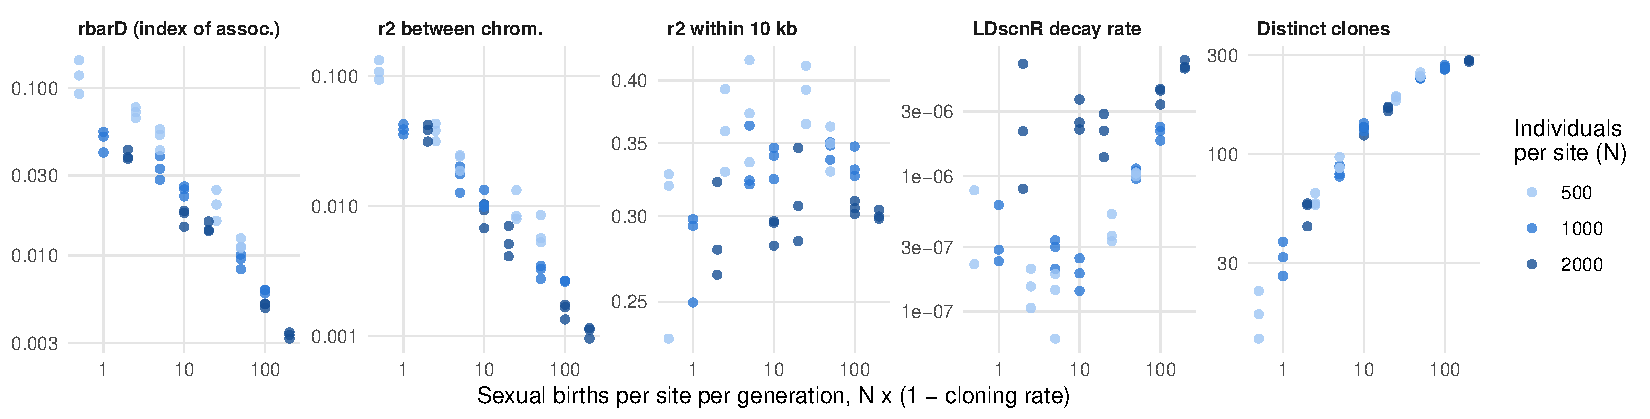
\includegraphics[width=\textwidth]{../figures/sexrate_ld.pdf}
\caption{LD summaries against the number of sexual births per site per generation, $N(1-c)$, for three population sizes $N$ ($c$ = cloning rate). Both axes are logarithmic.}
\label{fig:summaries}
\end{figure}

\textbf{Figure~\ref{fig:summaries}} shows three things:
\begin{itemize}\itemsep0pt
\item $\bar r_d$ and $r^2$ between chromosomes track the \emph{number} of sexual births, $N(1-c)$, very closely ($R^2 = 0.92$--$0.94$ on log scale). They cannot separate the rate of sex from population size.
\item LDscnR's within-chromosome decay rate behaves differently: it depends mainly on population size, explaining 58\% of the variation in log~$N$ compared with 37\% for $\bar r_d$ (cloning rates 0.9--0.995). It therefore carries the information needed to separate the two parameters.
\item $r^2$ within 10\,kb is saturated by clonal LD and carries almost no information.
\end{itemize}

\begin{figure}[h]
\centering
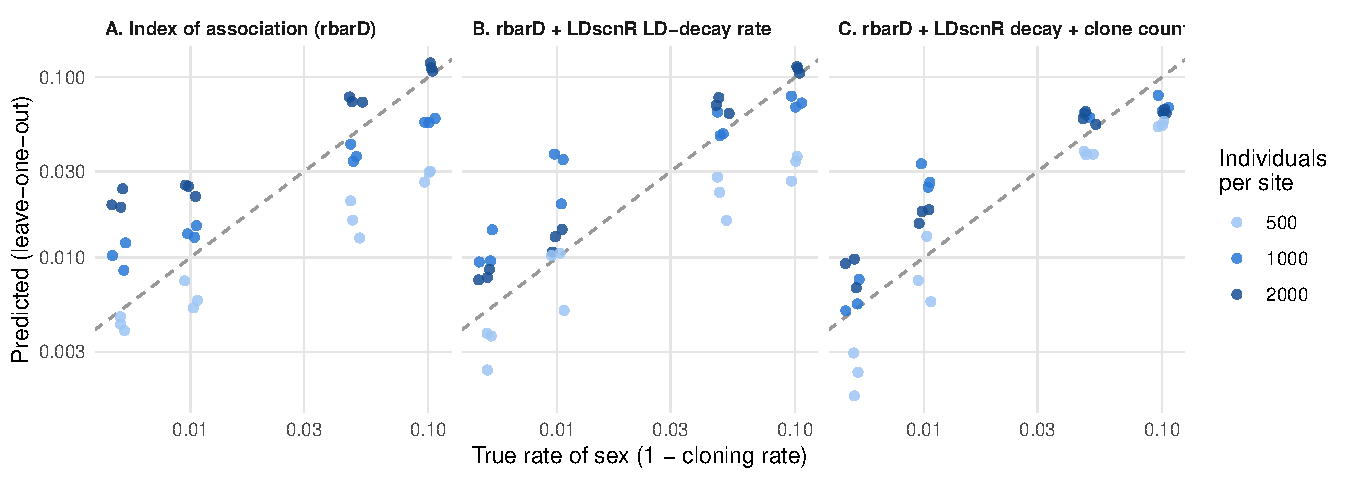
\includegraphics[width=\textwidth]{../figures/sexrate_loo.pdf}
\caption{Predicting the rate of sex $(1-c)$ for each simulation from the others (leave-one-out linear regression on log scale; cloning rates 0.9--0.995, 36 simulations).}
\label{fig:loo}
\end{figure}

\textbf{Figure~\ref{fig:loo}} turns this into a prediction test. With $\bar r_d$ alone, predictions stratify by population size and 61\% fall within a factor of two of the truth (RMSE 0.34 $\log_{10}$ units). Adding LDscnR's decay rate removes most of that stratification (75\% within a factor of two, RMSE 0.28), and adding the number of clones gives 86\% (RMSE 0.23).

\section*{Interpretation and next steps}

These results support the premise. A single LD statistic measures only the number of sexual events, while combining between-chromosome LD with distance-resolved LD decay separates the rate of sex from population size. ABC is the natural way to combine these statistics with others (diversity, the site-frequency spectrum, clone size distributions, loss-of-heterozygosity tracts) and to obtain estimates with uncertainty. We plan to:
\begin{enumerate}\itemsep0pt
\item build an ABC random-forest analysis on a few thousand SLiM simulations with priors on cloning rate, population size, migration, recombination and loss-of-heterozygosity rates;
\item validate it on simulated pseudo-observed data and quantify how much the LDscnR statistics add beyond $\bar r_d$;
\item test robustness to low sequencing depth and to non-random (outbreak-biased) sampling of isolates;
\item apply it to population-genomic data from Finnish \emph{S.~parasitica}.
\end{enumerate}

\textbf{Caveats.} These are 45 simulations from one model, analysed with simple linear regression rather than ABC; the numbers indicate feasibility, not final accuracy. The number of clones is a strong predictor here because isolates were sampled at random from populations at equilibrium. With samples biased towards outbreaks it will be less reliable, which makes LD-based statistics more important. LDscnR's decay fit failed at the most extreme clonality (cloning rate 0.999 with 500 individuals per site), but in that regime genome-wide LD already makes predominant clonality obvious.


\end{document}
